\RequirePackage[T1]{fontenc}
\documentclass[conference]{IEEEtran}
\usepackage{times}
\usepackage[numbers]{natbib}
\usepackage{amsmath,amssymb,graphicx,booktabs,array}
\usepackage{balance}
\usepackage[bookmarks=true,hidelinks]{hyperref}
\hypersetup{pdftitle={From Internal Writes to Action Changes: Prediction and Transfer in a Vision-Language-Action Policy},pdfauthor={},pdfsubject={},pdfkeywords={}}
\newcommand{\full}{\textsc{Full}}
\newcommand{\four}{\textsc{Four}}
\newcommand{\fourG}{\textsc{Four-G}}
\newcommand{\fullG}{\textsc{Full-G}}
\newcommand{\hp}{\textsc{HeadPos}}
\newcommand{\pool}{\textsc{Pooled}}
\newcommand{\norms}{\textsc{Norms}}
\newcommand{\sumread}{\textsc{Sum}}
\begin{document}
\title{From Internal Writes to Action Changes:\\Prediction and Transfer in a Vision-Language-Action Policy}
\author{Author Names Omitted for Anonymous Review}
\maketitle

\begin{abstract}
Can an internal edit's action effect be predicted before the edited output is generated? We study signed candidate-chunk changes in a frozen $\pi_{0.5}$ policy. Retaining signed, head-specific and action-position information improves some capacity-controlled comparisons, but does not establish stable transfer across task cohorts. With matched nonlinear estimators, complete algebraic write proxies have 0.52\% higher contrast error than compressed proxies across four historical initialization clusters; coordinate-level exceptions remain. Native calibration separates proxy fidelity from realized writes, while optimal per-axis signed rescaling leaves 57--81\% median residual energy between pulse and persistent effects. A bounded simulator continuation then connects saved pulse commands to motion: after an exact none repeat, shared and random edits yield final end-effector distances of 7.65 and 35.74~$\mu$m from none over 0.25~s at one state. Equal gripper targets coexist with unequal joint positions. The evidence separates local representation value, command effects and short-window motion from transferable prediction and task benefit.
\end{abstract}
\IEEEpeerreviewmaketitle

\section{Introduction}
An internal edit can alter a robot policy's action chunk without making its direction, timing or task dependence predictable. Intervention-based explanations and policy correction therefore require more than showing that an activation change affects output.

We study the flow-based vision-language-action (VLA) policy $\pi_{0.5}$~\citep{pi05} on LIBERO~\citep{libero}. Given a snapshot and visual-content edit, we predict the signed edited-minus-unedited action chunk from the unedited first-call computation. The target is the edit's effect, not ordinary action decoding.

Prediction may fail because compression loses sign, head or position structure, or because richer inputs increase estimation difficulty without a transferable mapping. Persistent edits also change later reads: their effects need not scale a single pulse.

We test capacity-controlled task transfer, matched nonlinear estimators and native pulse/persistent continuation (Fig.~\ref{fig:overview}), then execute a bounded saved-command contrast. Only the first comparison evaluates excluded task cohorts.

Signed structure has conditional predictive value; nonlinear compression removes an apparent full-dimensional advantage. Nonuniform generation effects and small simulator motion then distinguish measurable intervention effects from transferable prediction or task benefit.

\begin{figure*}[t]
  \centering
  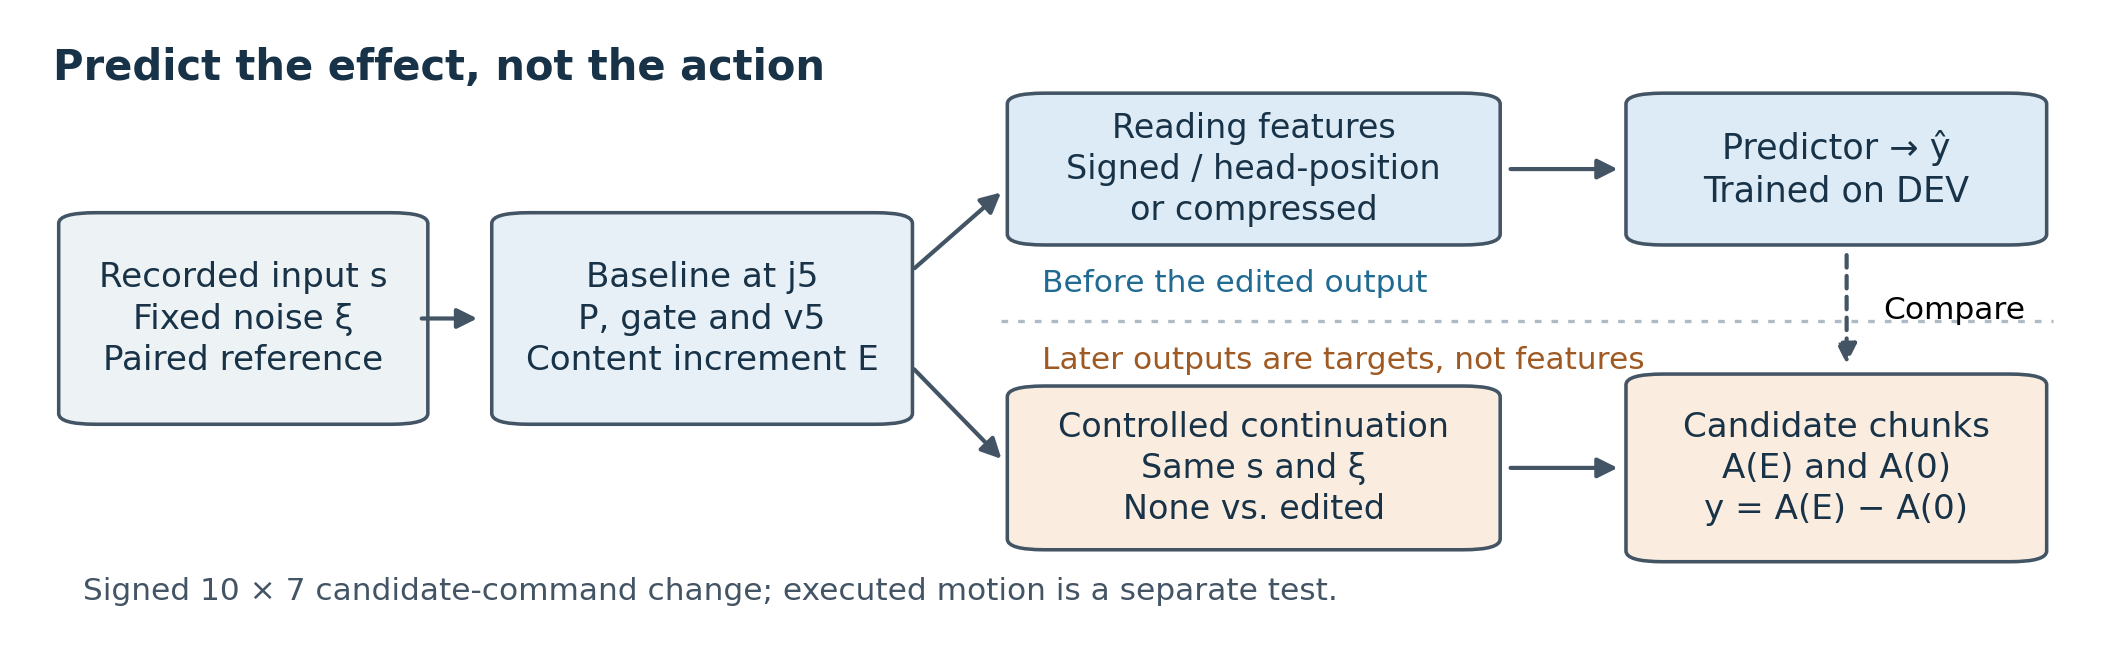
\includegraphics[width=\textwidth]{figures/F1-OVERVIEW.png}
  \caption{\textbf{Predicting an edit's action effect.} Unedited first-call reads and shared context predict the signed candidate-chunk difference. Edited continuation lies beyond the information cutoff. Three tests examine representation/capacity across tasks, estimator choice within represented tasks, and pulse/persistent continuation. This is a conceptual diagram; candidate commands, issued commands, and motion remain distinct.}
  \label{fig:overview}
\end{figure*}

\section{Related Work}
\textbf{Interpreting and steering VLA policies.}
VLA interventions include FFN steering with random controls~\citep{haon2025}, activation injection/action decoding~\citep{grant2026}, behavior tracing~\citep{shi2026} and closed-loop feature control~\citep{observing2026}. We instead predict a signed edit effect before observing its output.

\textbf{Behavioral sensitivity and generalization.}
ReSteer~\citep{resteer2026} studies instruction-switch steerability and paired-data refinement; \citet{zhang2026} connect visual masking, action discrepancies and generalization. We test directional, same-snapshot edit contrasts; intervention and execution themselves are not claimed innovations.

\textbf{What a probe comparison establishes.}
Probe controls separate fitting flexibility from generalizable information~\citep{hewitt2019}. We compare linear effective degrees of freedom (EDF) and matched nonlinear compressed controls. Equal EDF or numerical penalties constrain comparisons without equating hypothesis classes.

\section{Predicting the Effect of an Internal Edit}
\label{sec:method}
\subsection{Target and information available to the predictor}
Let $s$ be a recorded policy input and generation state, $\xi$ fixed generation randomness, $E$ a content increment, and $\sigma$ its application schedule. The response is
\begin{equation}
 y_{\sigma}(s,E)=A_{\sigma}(s,E;\xi)-A(s,0;\xi)
 \in\mathbb{R}^{10\times7},
 \label{eq:target}
\end{equation}
where $A$ contains three translation, three rotation, and one gripper command per position. These are quantile-unnormalized LIBERO controller inputs, not measurements in meters or radians. Each intervention has its own unedited baseline. Candidate commands are not measured motion or task success.

Index $j$ denotes ten zero-based Euler solver calls, distinct from command positions. Edits enter layer~9 at $j5$, persist through $j9$ in prediction studies, or pulse only at $j5$. The realized increment is $E=\operatorname{fp32}(V_{\rm mod})-\operatorname{fp32}(V_T)$ for stored BF16 modified/perturbed-prefix values. Paired clean/perturbed references and the unedited pass are privileged inputs: prediction starts at $j5$, not before generation.

Each paired key-background comparison fixes the realized increment; increments can vary across snapshots. ``Shared'' names a construction, not one vector reused in every state. Prediction is conditional on the snapshot and specified edit.

At the first intervention call $j=5$, eight query heads sharing one KV head read $r_{hp}=P_{hp}E$ at position $p$, retaining the complete-softmax denominator. Their projected, gated sum is
\begin{equation}
 \widetilde w_p=g_{\tau}\odot\sum_{h=1}^{8}r_{hp}W_h^O .
 \label{eq:write}
\end{equation}
where $P_{hp}$ is unedited attention, $W_h^O$ the head's output projection, and $g_\tau$ the gate. \full\ uses this complete $10\times1024$ FP64 algebraic proxy, preserving position/sign but summing heads; it is not the realized native residual write. Calibration compares its pre-gate sum with native output change $\Delta O$, and $\widetilde w$ with post-attention residual change $\Delta H$. All predictors share natural information through $j5$, including flow vector field $v_5$; edited outputs and later natural endpoints are excluded.


\subsection{Representations and capacity controls}
Task-transfer predictors share nine context coordinates: four principal components of paired unedited $(x_0,v_0,x_5,v_5)$ and proprioceptive state, four of $v_0^T-v_0^C$, and policy-step index divided by 520. Here $x_j$ is the flow state and $v_j$ its vector field. \four\ adds four retained write coordinates; \full\ adds the complete proxy; \pool\ substitutes a pooled reader. \hp\ retains signed reads by head and position, \norms\ their 80 magnitudes, and \sumread\ their signed 256-vector sum. Context-only, four-norm, and pooled-four controls complete nine families.

Weighted ridge has an unpenalized intercept. Added-feature scales use fitting queries; original context/target scales stay fixed. Penalties $0.1,1,10$ are reported without evaluation selection. A separate comparison matches training EDF, including the intercept, to \four\ at penalty~1; geometry can still differ.

Grouped \fourG/\fullG\ share 40 arm-context/dose features and four unpenalized arm intercepts, adding four non-whitened write PCs or the full proxy (44 penalized inputs for \fourG). Read blocks use one training RMS scale. Linear/RBF ridge share three penalties. RBF uses representation-specific training-median bandwidths or, for sensitivity, the full-input bandwidth. All PCA/readers/scales are fitted within training folds.

\begin{figure*}[t]
  \centering
  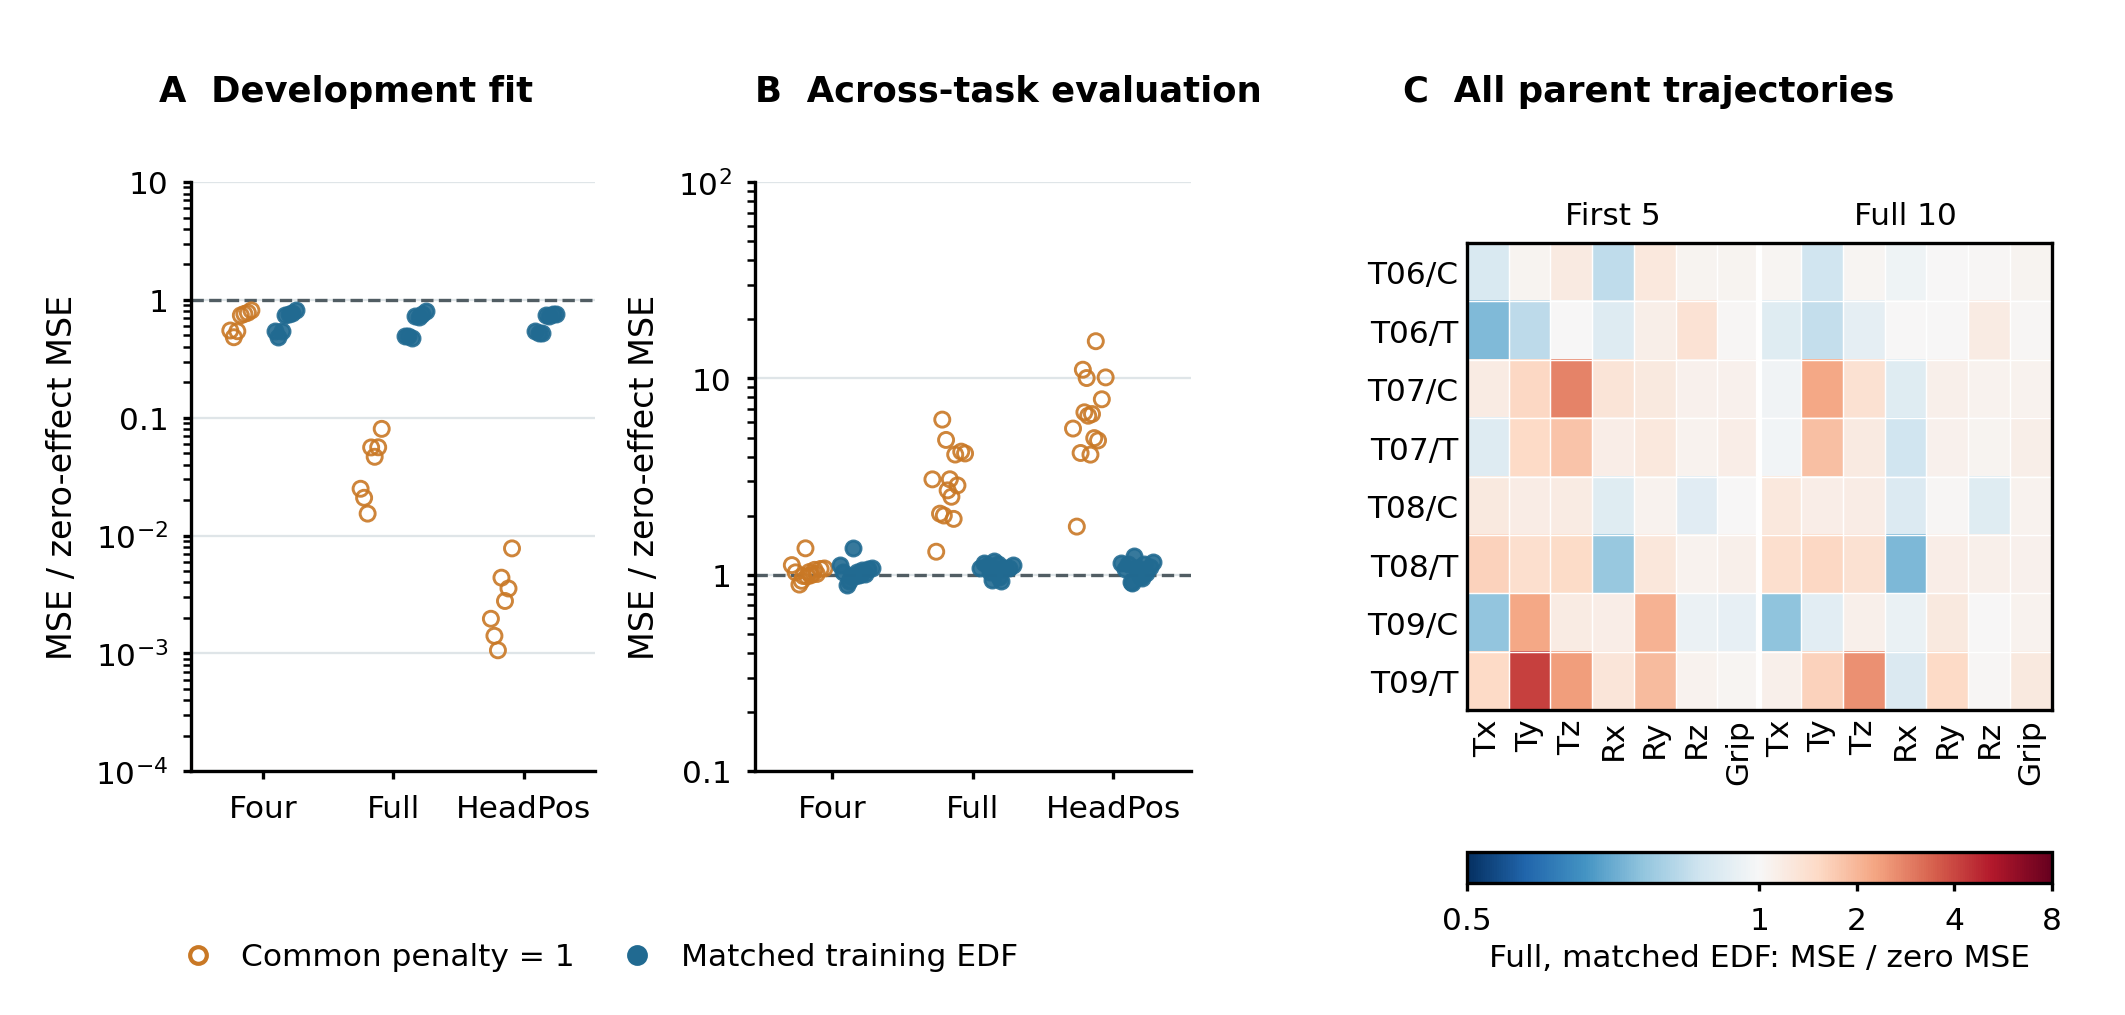
\includegraphics[width=\textwidth]{figures/F2-CAPACITY-TRANSFER.png}
  \caption{\textbf{Fitting well does not establish transfer across task cohorts.} \textbf{A:} development loss/zero for all seven coordinates. \textbf{B:} evaluation loss/zero for both C/T populations and all coordinates, comparing \four, \full, and \hp\ at common $\lambda=1$ and matched training EDF. A,B use all ten positions; all panels use frozen development per-position scaling. Each ratio uses its own population's zero baseline; coordinates are never averaged across physical units. \textbf{C:} all eight evaluation trajectories, both overlapping windows, and seven coordinates for EDF-matched \full\ (112 cells). Training and evaluation populations are distinct.}
  \label{fig:capacity}
\end{figure*}

\subsection{Evidence populations}
Task-transfer fitting uses 48 shared-edit queries from two tasks/four trajectories; evaluation uses 96 queries from four other tasks/eight C/T trajectories. C/T is the clean/perturbed trajectory, not internal key background. Camera parameters and visited states also change, preventing attribution to task alone. Twenty-four overlapping anchors support key contrasts. Previously inspected cohorts are not a new blind test.

The grouped study uses 192 persistent labels at 48 queries: shared, random-matched, distance-matched and full-value-restoration. Four initializations give two clusters per task. Outer leave-one-initialization-out folds group queries/arms; the task remains represented. Inner grouped validation selects penalties for individual-arm prediction or the contrast
\begin{equation}
 d_{\sigma}(s)=y_{\sigma}(s,E_{\rm shared})
              -y_{\sigma}(s,E_{\rm random}).
 \label{eq:contrast}
\end{equation}
Predictions are differenced before scoring. This is persistent-effect initialization transfer, not pulse or held-task validation; some inner training folds contain only the other task.

The native diagnostic uses 24 snapshots from four tasks/eight paired C/T trajectories, at queries 11/16/22 and layers 1/9/18. None (N), shared pulse (S) and persistent (P) share graph $G^\star$, receiver $K_T$ and saved FP32 noise. Stock-policy endpoint/noise equivalence is unassumed; paired trajectories are not independent initializations.

A development pilot uses queries 11/22 from four initializations, collecting shared/random pulses and shared persistent effects against their own $G^\star$ none. Its 72 generations include none repeats, both zero-edit schedules and delayed S/P repeats; R has no delayed repeat. Eight pulse pairs are qualified, not task transfer.

\subsection{Scoring and units of evidence}
Task-transfer MSE averages positions, within-trajectory queries and tasks equally per parent, separately by coordinate. MSE/zero-effect MSE below one beats zero. Native and development-scaled scores remain. Two parents, two overlapping windows (first five/all ten) and seven coordinates give 28 cells.

The grouped summary averages training-standardized first-five error over coordinates, initializations and tasks equally; native errors stay separate. Gains use identical fold scales. Coordinates, adjacent queries and overlapping windows are dependent; undefined denominators remain. This small study cannot support a powered population null. A source-based diagnostic maps saved commands through arm clipping/scaling and gripper sign; it executes no environment.



For one coordinate over $m$ positions, let $\delta_S=S-N$ and $\delta_P=P-N$. The three archived effect RMS values recover their inner product:
\begin{equation}
\langle\delta_S,\delta_P\rangle
=\frac{m}{2}\bigl(R_S^2+R_P^2-R_{P-S}^2\bigr).
\end{equation}
The best signed gain $\alpha^*=\langle\delta_S,\delta_P\rangle/\|\delta_S\|^2$ leaves a fraction of persistent-effect energy
\begin{equation}
\rho=\min_{\alpha\in\mathbb R}
\frac{\|\delta_P-\alpha\delta_S\|^2}{\|\delta_P\|^2}
=1-\cos^2(\delta_S,\delta_P).
\end{equation}
This response-visible projection allows reversal; it is not prediction. Zero denominators remain undefined. A $10^{-10}$ moment tolerance checks numerical sensitivity, not repeat noise or importance. Residuals may include offsets without temporal reordering.

\begin{figure*}[t]
  \centering
  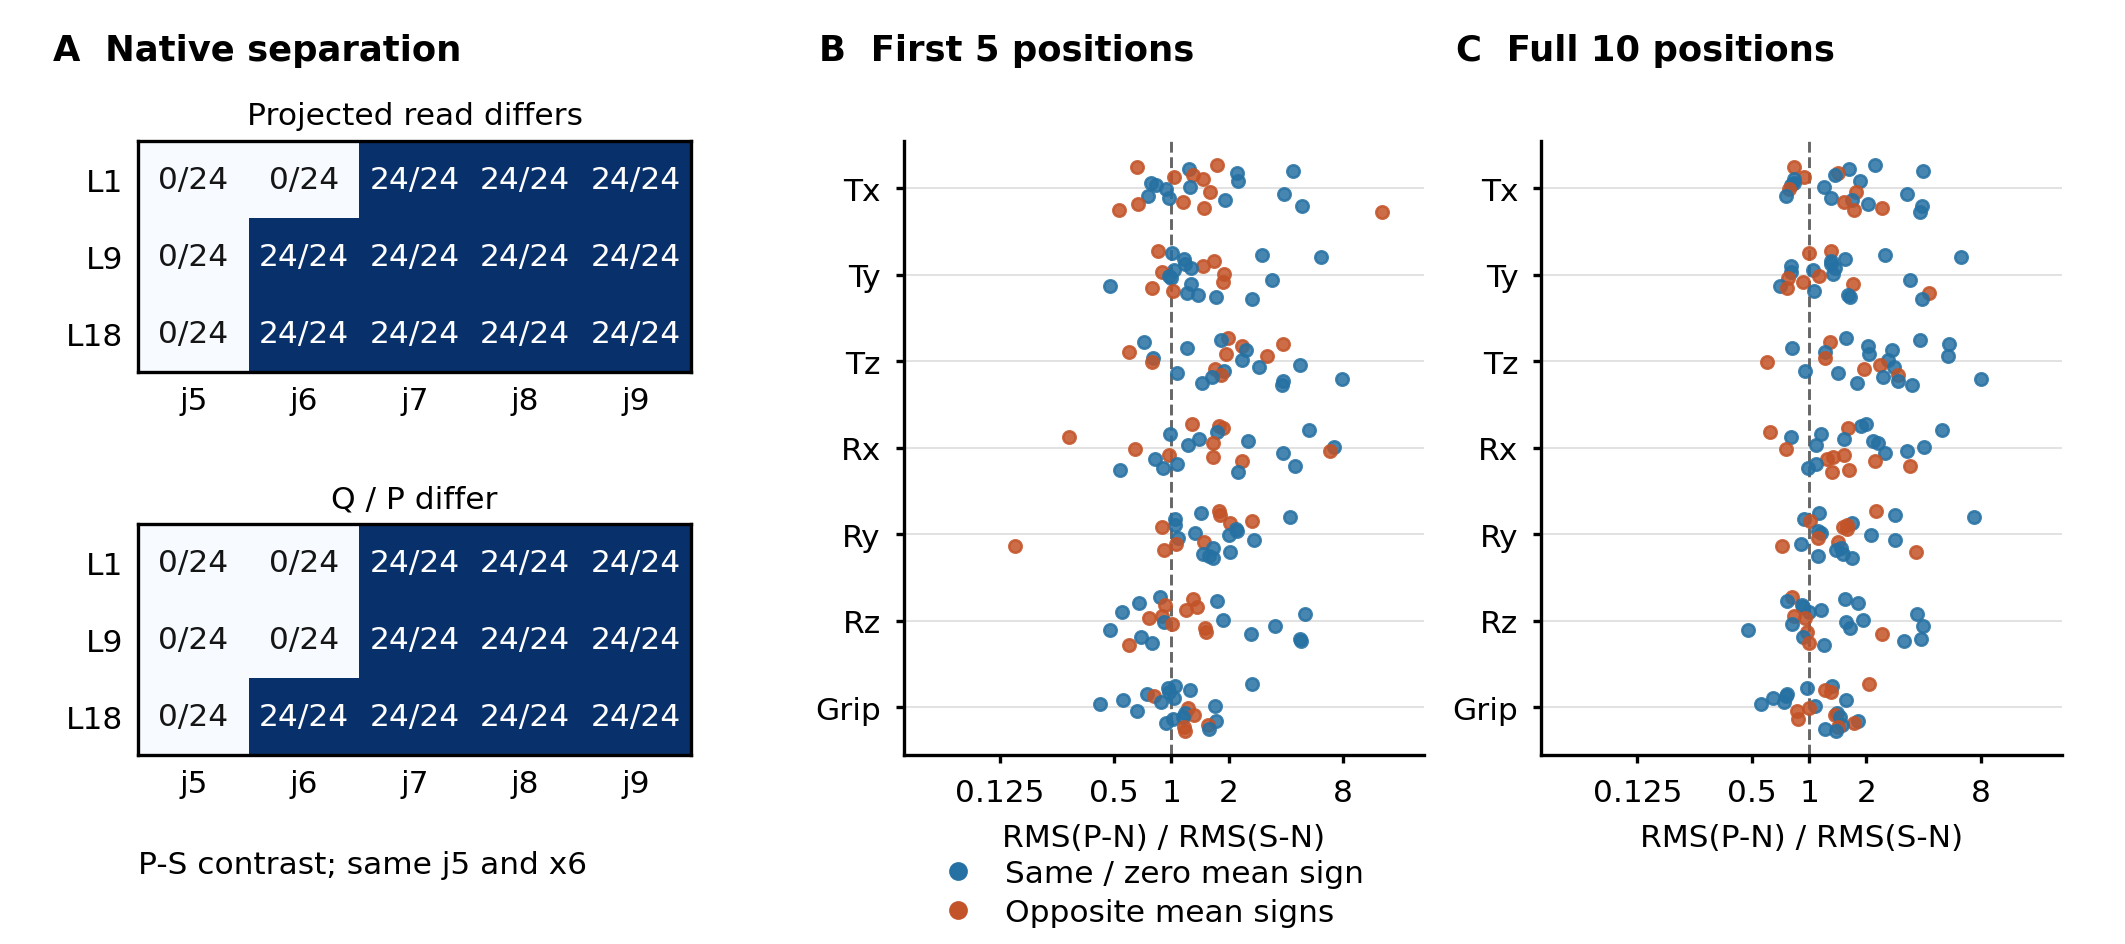
\includegraphics[width=\textwidth]{figures/F3-NATIVE-PVP.png}
  \caption{\textbf{Sustained editing is not uniform pulse amplification.} \textbf{A:} two aligned layer-by-flow matrices count differences among 24 snapshots: pre-gate projected attention output and queries/attention probabilities (Q/P). At $j6$/layer~9 the former differs while Q/P agree. \textbf{B,C:} every snapshot's persistent-to-pulse endpoint-effect RMS ratio, separately by coordinate, for first-five/full-ten windows. Color marks opposite signed window means, not pointwise reversal. Both effects use the same none baseline. Dependent observations remain visible; ongoing exposure and dynamics are confounded.}
  \label{fig:native}
\end{figure*}





\section{Results}
\label{sec:results}
\subsection{Does retaining reading structure improve task transfer?}
Richer features sharply reduce fitting error while increasing effective capacity. At $\lambda=1$, EDF is 6.386 for \four, 39.177 for \full, and 45.763 for \hp. Full-chunk development error/zero ranges across coordinates from 0.482--0.815, 0.015--0.080, and 0.001--0.008, respectively.

The ordering reverses on evaluation tasks (Fig.~\ref{fig:capacity}). \full\ loses to \four\ in every primary cell at all three penalties. At penalty~1 it also loses to zero and context-only throughout, with error/zero ratios of 1.303--9.019.



EDF matching reveals conditional benefits. Current reading beats pooling in 25/28 cells; signed head-position reads beat magnitudes in 20/28 and signed summation in 24/28. Yet \full\ beats \four\ in only 11/28 and zero in 7/28. None of its favorable comparisons with \four\ improves in all four tasks.

These advantages support current reading and signed structure under the estimator; they do not establish superiority to zero or stability across tasks.

\full\ worsens translation-z and rotation-y versus \four\ in every parent/window panel, including all four tasks for perturbed-parent first-five prediction. \hp\ worsens gripper error versus \full\ throughout. Conversely, clean-parent full-ten rotation-x beats zero in all four tasks (ratio 0.944), but \four\ in only three. No uniform ranking emerges.

Changing keys while holding the edit fixed produces nonzero endpoint interactions at all 24 anchors, yet EDF-matched \full\ beats \four\ in only 8/28 clean-key cells. Interaction prediction is also mixed: perturbed-parent first-five translation-x/y/z ratios are 0.944/0.878/0.833 for \four\ and 0.985/0.917/0.813 for \full.



\subsection{Does compression explain the prediction gap?}
Within the two represented tasks, selected linear \fullG\ improves first-five persistent-contrast error by 3.49\% over zero but only 0.20\% over \fourG, with two favorable initializations. It loses to \fourG\ at every common penalty. RBF \fullG\ improves 0.98\% over selected linear \fourG, a comparison changing both representation and estimator.

The matched nonlinear control changes the interpretation (Table~\ref{tab:kernel}). Full-write error is 0.524\% higher than compressed-write error with individual training-median bandwidths, and 0.320\% higher with a common bandwidth. All four initializations favor compression under both selection objectives and all three fixed penalties. Full-RBF's earlier advantage therefore does not demonstrate value in additional dimensions.

\begin{table}[t]
\centering
\caption{Grouped first-five persistent-contrast prediction. Gain is $(L_{\rm baseline}-L_{\rm candidate})/L_{\rm baseline}$. Penalties are selected within training folds. Four deterministic initialization clusters; these are descriptive comparisons.}
\label{tab:kernel}
\begin{tabular}{@{}p{0.53\columnwidth}rr@{}}\toprule
Candidate versus baseline & Gain & Favorable\\\midrule
Linear \fullG\ versus linear \fourG & $+0.197\%$ & 2/4\\
RBF \fourG\ versus linear \fourG & $+1.498\%$ & 4/4\\
RBF \fullG\ versus RBF \fourG & $-0.524\%$ & 0/4\\
Same, common bandwidth & $-0.320\%$ & 0/4\\\bottomrule
\end{tabular}
\end{table}

Exceptions remain: full features improve 27/56 initialization--window--coordinate cells; compressed RBF loses to zero in 10/28 first-five cells. Its 1.50\% gain over linear \fourG\ depends on tuning: common $\lambda=0.1$ instead increases contrast error 0.32\% and individual-arm error 3.31\%. Estimator and regularization both change.

Extra dimensions are unnecessary for this diagnostic's gain; this is neither causal irrelevance, equivalence nor cross-task generalization.

\begin{figure*}[t]
\centering
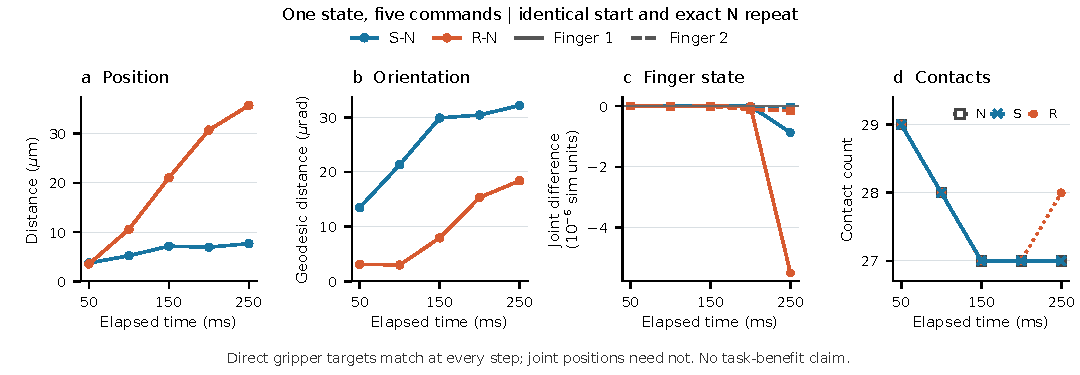
\includegraphics[width=\textwidth]{figures/fig_physical_response.pdf}
\caption{\textbf{Command differences reach motion with mixed S/R ordering.} All five times at T00/R00/q11 show position/orientation distance from N, signed finger-joint differences and contact counts. Starts match and N repeats exactly. Equal gripper targets coexist with unequal joint positions; R ends with 28 contacts versus N's 27. One state, 0.25~s, no policy feedback or task-benefit claim.}
\label{fig:physical}
\end{figure*}

\subsection{Does sustained editing simply scale the pulse effect?}
Pulse and persistent schedules agree through $j5$ and next flow state $x_6$ in all 24 snapshots (Fig.~\ref{fig:native}). At $j6$/layer~9, queries, attention probabilities, gates, and incoming residuals still agree, while renewed editing changes projected attention output before gating in every snapshot. Queries and probabilities diverge at layer~18 of that call and at all three measured layers by $j7$.



First-five persistent RMS is smaller in 48/168 snapshot--coordinate cells and larger in 120, with no ties; signed window means are opposite in 63. Full-ten counts are 42 smaller, 126 larger, and 56 opposite. Thus persistence does not uniformly strengthen the pulse effect.

Allowing each snapshot and coordinate its own optimal signed gain still leaves median residual energy fractions of 57.5--80.9\% for first-five and 67.3--81.3\% for full-ten effects. All 336 projections are numerically defined without moment correction. The result is heterogeneous: first-five translation-y includes a nearly collinear case with only 0.0358\% residual energy. These fractions quantify departure from pure gain, including possible additive offsets; they neither measure physical importance nor prove altered centered temporal patterns.



The additional output precedes receiver disagreement. Repeated exposure and dynamics remain confounded: this neither isolates feedback nor explains prediction error or first-call insufficiency when schedule is known.

The development pilot passed 72 native calls and qualified 16 shared/random pulse labels. Both pulse effects and their contrast have nonzero first-five RMS per coordinate in all eight snapshots (Table~S1); positions can still be zero. Shared exceeds random in only 3--5/8 snapshots per coordinate. Global edit norms differ by up to 5.318 parts per million; none matches exactly. These contrasts are numerically observable, without a uniform amplitude ranking or prediction guarantee.

Archived $G$ reconstruction passes 40/40 cache checks; pilot $G^\star$ T-reader proxies differ in 16/16 comparisons and own-baseline persistent effects in 112 dependent cells. First-five discrepancy exceeds new shared-pulse RMS in 40/56 same-coordinate cases (Fig.~S1). This does not explain earlier cross-task error or invalidate within-$G^\star$ contrasts. Fresh clean-C flow and the numerical cause remain unmeasured.

Within $G^\star$, 192 pre-site checks match (12 fields, 16 S--N/R--N pairs). Full-ten native-norm relative errors are 1.30--7.02\% pre-gate (cosine $\ge0.997532$) and 9.63--57.49\% gated (Table~S2). T01/R00/q11 R reaches 88.43\% at $p=0$; full-ten matching signs at 6696/6711 jointly nonzero coordinates coexist with 3529/10240 native-zero/proxy-nonzero coordinates. The larger gate/residual term and signed cross terms are algebra, not causal attribution. Near-equal-E total effects remain valid; matching native dose changes the question. This calibration explains neither earlier prediction nor cross-graph gaps.

Controller mapping adds an endpoint boundary. First-five S--R gripper values differ in 29/40 comparisons, yet all 40 signs agree (Table~S3). Both pulse-versus-none contrasts preserve signs; every nonzero arm difference survives clipping/scaling. Equal gripper targets require equal initial memory/update counts and do not imply equal finger motion.

\subsection{Do saved command differences reach motion?}
At T00/R00/q11, each branch replays ten settling steps and 55 original parent commands from the original initialization. After source-path qualification, matching declared/critical/physical starts and an exact full-trajectory N repeat gate S/R. Five cached commands execute at 20~Hz (0.25~s), without inference or feedback. The retained N recorder-close failure stays failed; verified observations alone are reused (Tables~S4--S5).

Position differences are nonzero at all five times (Fig.~\ref{fig:physical}), ending at 7.65~$\mu$m for S--N and 35.74~$\mu$m for R--N; S decreases at time four. S instead has the larger final orientation difference (32.17 versus 18.39~$\mu$rad). Equal gripper targets coexist with unequal joint positions; R's last contacts are 28 versus N's 27. No branch terminates or succeeds within the window; that is not task failure or evidence of benefit.

\balance
\section{Discussion and Next Tests}
One policy, retrospective cohorts, four development initializations and one physical state limit generality. Local motion neither explains prediction failure nor isolates write dose or task benefit.

Pulse prediction needs same-graph features/labels and matched context, capacity and nonlinear controls. Test new initializations and excluded tasks with matched Camera operator, clock, schedule and target. Group by initialization; preregister useful gains and assess uncertainty at initialization/task level. Longer execution must connect predictions to object/task consequences; technical replay and micrometre motion do not substitute.

\section{Conclusion}
Signed structure has conditional predictive value, without stable full-write transfer. Persistent effects are nonuniform, and qualified local motion is small with mixed S/R ordering. Independent prediction and task relevance remain open.

\clearpage
\interlinepenalty=10000
\bibliographystyle{plainnat}
\bibliography{references}
\end{document}
